Mobile consumer-electronics devices, especially phones, are powered from batteries that are limited in size and therefore capacity. This implies that managing the battery power is paramount in such devices. As long as the battery technology continues its slow pace of improvement, the only viable approach is to reduce the amount of energy required to provide specific services. Two of the most power consuming services on a smartphone are network and wireless data. Though internet connectivity is important, the nature of data transfer does not require uninterrupted service. We take advantage of this fact to cut off power to these modules when it is not required. The challenge is to predict, when the users require these services and when they do not. Existing solutions usually schedule the services based on fixed hand-coded rules that do not work for all users or usage scenarios.  In this paper, we propose an activity-based model that uses machine learning approaches to intelligently schedule Wi-Fi according to a user's activity level. Several higher order features from the raw sensor data stream are used to classify the activity level. Two aspects of the problem are considered, namely the accuracy of estimating the activity level as well as the power required in sensing and estimation. Experimental results on Android based smartphones demonstrate that an active user can get up to 37\% increase in battery life without significant effect on the user experience.

\section{Introduction}
A smartphone is a mobile phone built on a mobile operating system, with higher computing capability
and connectivity options compared to a feature phone. Inclusion of features such as accelerometers,
GPS, compass, radio receivers, cameras and audio processors have made smartphones the primary
device for personal assistance including communication, navigation, entertainment, imaging and
information access. By far the most significant
problem with most smartphones is their highly limited battery life. In recent times, hardware
manufacturers have worked extensively to solve this problem, resulting in highly energy efficient
processors and some promising directions in power-efficient displays. However, the wireless communication modules continue to consume significantly more energy in comparison and is a potential  source for energy savings.

%\begin{center}
%\begin{figure}[t]
%\centering{
%\includegraphics[width=1\columnwidth]{description.png}
%\caption{Example of Wi-Fi service scheduler. The service is scheduled based on the user's activity. Dark red color indicated that Wi-Fi is turned off during that time.}
%\label{fig:sampleschedule}}
%\end{figure}
%\end{center}

Today's internet is the mobile internet. People are moving towards smart-phones for general browsing, social networking and emails etc. Figure \ref{fig:bar} shows the percentage of phone owners who used internet or email on their phone. 56\% of smartphone users use their phones, not their PCs or tablets, as their main way to access the internet. Thus reducing the energy consumed by the network processes like Wi-Fi on smartphone devices could help in huge energy savings.

\begin{center}
\begin{figure}[ht]
\centering{
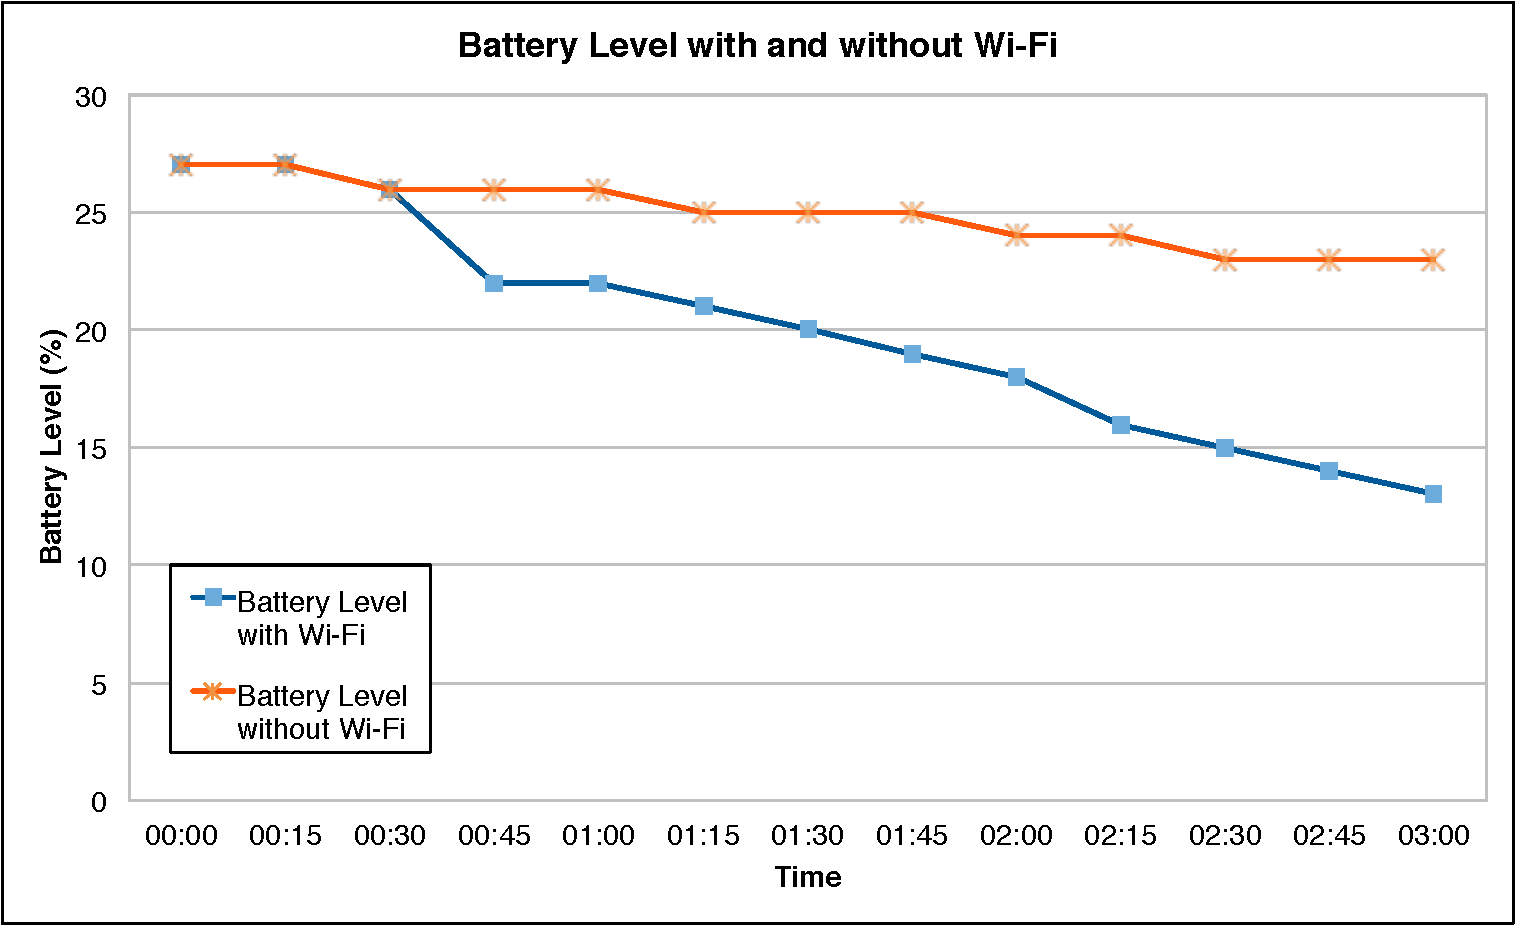
\includegraphics[width=0.8\columnwidth]{batteryvariations.pdf}
\caption{Battery level variation on a smartphone with and without Wi-Fi enabled (Data transfer: 2KB at 5 minute intervals).}
\label{fig:variations}}
\end{figure}
\end{center}

An interesting nature of wireless data communication arises the connectionless protocols used for
data communication. The data is buffered at different points in the communication path and is delivered
whenever a connection to the device is available. Moreover, most usage patterns involve intermittent
periods of activity and inactivity. We take advantage of this fact to switch off the wireless data radio,
whenever the usage is not significant. This would result in significant savings of power is used appropriately.
However, there are two challenges that need to be addressed to achieve this. We need to be able to
predict periods of activity and inactivity of the specific user to shut down the wireless appropriately.
Inaccuracies in this prediction will result in a poor user experience or a lost opportunity for power saving.
On the other hand the data collection for determining the user state and the classification process should
be simple enough to avoid excessive energy usage for its purpose, nullifying any savings resulting
from powering off the wireless.

\begin{figure}[h]
\centering
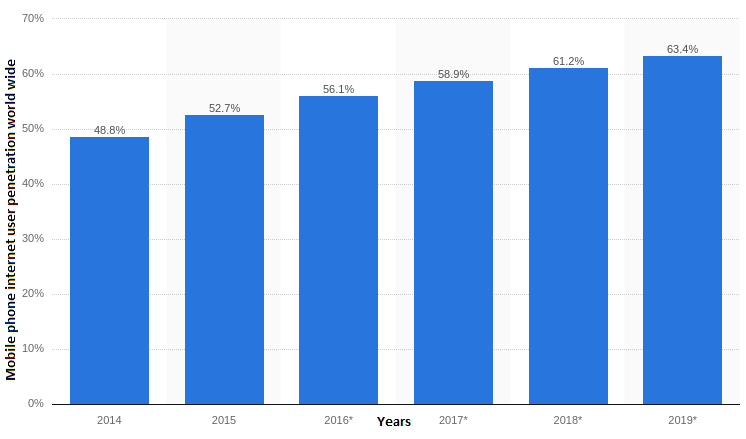
\includegraphics[width=0.9\columnwidth]{bar_01.png}
\caption{World wide percentage of mobile phone users and prediction, who use internet or email on their phone in $2014-2019$\cite{survey}.}
\label{fig:bar}
\end{figure}

\subsection{Contributions}
In this work, we look at modeling and monitoring the user activity level(via machine learning) to decide when the wireless data
modules should be turned off for maximal energy saving without compromising the user experience.
The Wi-Fi scheduling is formulated as a classification problem, where Wi-Fi is scheduled based on the predicted usage of the user in the next time window.
The specific problems that we deal with in this work may be summarized as:
\begin{itemize}
\item \emph{Activity Modeling on Smartphone:} We propose a power-efficient approach to modeling the
user's activity level on the smartphone device using various sensors and parameters that are easily available
on most smartphones.
\item \emph{Energy Reduction by continuous Activity Scheduling:} We proposed an approach to schedule
continuously running processes like Wi-Fi for better energy management without hampering the user experience.
\end{itemize}

We first take a look at the existing works in the area of activity classification and energy efficient mobile computing to understand
the popular approaches in this area, which are then leveraged in coming up with an efficient way of
activity modeling.

\subsection{Related Work}
Mobile phone based pattern recognition and data analysis has been a hot research field in the last decade.
Specifically, the area of modeling user behavior to provide location, time and need based services has seen
significant attention. Most smartphones are filled with a variety of applications that use sensors to measure
movement and understand the world around us. They can be programmed to teach itself to work better, based
on how you use it, the applications you run, and how you use it to communicate with others.

A lot of work has also been done on activity and gesture recognition with the help of accelerometer sensor
data. Sun {\em et al.}~\cite{Sun} proposed a mechanism to classify physical activities of the bearer of the device
using accelerometer data with varying positions and orientations. The embedded tri-axial accelerometer in a
mobile phone can continuously log the experienced forces at each sampling interval and produce 3-D
acceleration reading $A$ = ($a_x$,$a_y$,$a_z$) along three orthogonal axes. In addition to the raw sensor
data, several features derived from the accelerometer sensor including mean, variance, correlation, energy,
frequency-domain entropy, cepstral coefficients, and log-FFT frequency bands~\cite{bao,lester,ravi,maurer,lester2,wu,rai,weiss}.
Further, Longstaff {\em et al.}~\cite{longstaff} proposed different health related applications via semi-supervised
activity modeling on smartphone. Realizing the effectiveness of accelerometer data in determining various usage
parameters, mobile phone manufacturers have started embedding dedicated low-power motion sensor processors
in addition to the main CPU on smartphones and tablets. In this work, we use accelerometer based features that
were proved good by most of these methods for modeling the user activity. Along with accelerometer data, we
also took other important indicators that suggest the type of user activity such as user interaction, and CPU and RAM
usage on the device. A detailed description of the specific features that are used is given in Section~\ref{sec:Features}.

Activity traces can improve the user interface mechanisms across a range of applications. For example, they can
be used as automated reminder or triggered for an action or input at a convenient moment~\cite{elder}. Recently,
researchers have started applying various machine learning approaches to activity recognition on smartphones.
Yan {\em et al.}~\cite{yan} proposed an efficient continuous activity recognition system. They tried to model
continuous user activity in a Markovian model based on the currently recognized activity. Zhuang {\em et al.}~\cite{location}
looked at the problem of energy-efficient location sensing on a smartphone. They tried to find the location using
substitution, suppression, piggybacking and adaptation methods, thus avoiding the use of power intensive
sensors like GPS for getting the location. Unlike the above works that tries to do a specific task in an efficient
manner, we use a combination of activity recognition and intelligent scheduling to save power dissipation by
the most power hungry processes on a typical smartphone.
Towards this, we present a more detailed analysis of the aspects of the phone that consumes the most
amount of power (in Section~\ref{sec:WCP}). This is followed by a description of our approach and the
activity classification model. In Section~\ref{sec:Exp}, we provide the results of various experiments
comparing our approach with the base case of regular usage profiles.

\section{What consumes Power?}
\label{sec:WCP}
Different applications have different power requirements. Figure~\ref{fig:chart} shows the relative power consumed by various services and applications on a smartphone device. It can be clearly observed that network services such as
Wi-Fi, EDGE and 3G are most power consuming processes on the device, and of the three, Wi-Fi is the worst offender.
However, in idle mode, Wi-Fi consumes very less power.

\begin{figure}[ht]
\centering
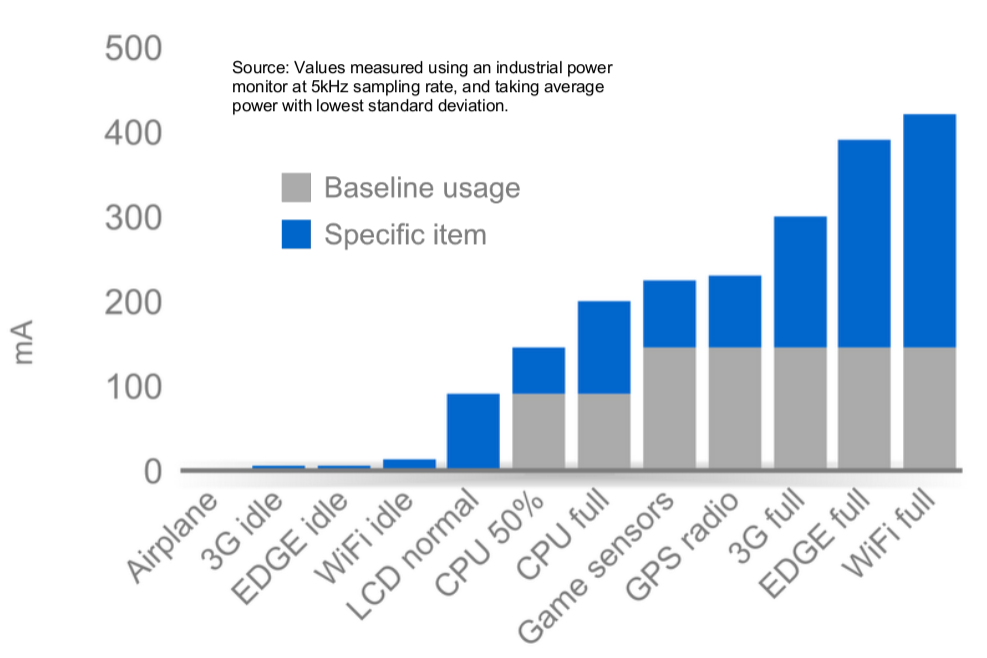
\includegraphics[width=0.9\columnwidth]{powerConsumption.png}
\caption{Component-wise energy consumption on Android (Jeff Sharkey~\cite{bworld}).}
\label{fig:chart}
\end{figure}

The power consumed by the network services also varies with the duration between data transfer operations.
%Table~\ref{tab:bundle} and
Figure~\ref{fig:pie}  shows the power consumed by the service when bundled transfer
mode is used, compared to unbundled data transfer mode. In our experiments, the energy consumed
by unbundled transfer was up to 3 times that consumed by bundled transfer.

\begin{figure}
\centering
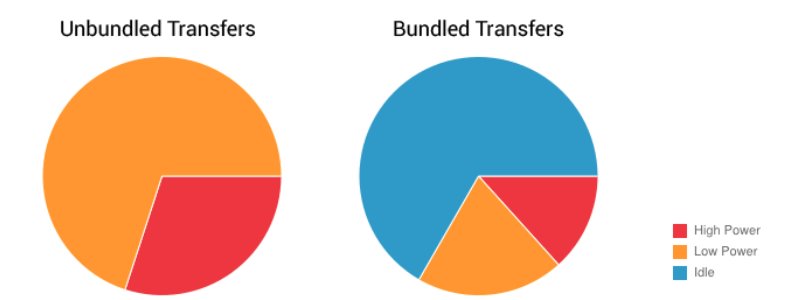
\includegraphics[width=0.9\columnwidth]{BundledPie.png}
\caption{Duration of time spend under different states (high power, low power and idle) by applications under Bundled and Unbundled packets transfer mode (Kumar Rangarajana~\cite{battery})}
\label{fig:pie}
\end{figure}

The best practices for the network applications is to fetch as much data as possible in one go. Google recommends pre-fetching data that will initiate in next 2 to 5 minutes, and in order of 1-5 MB. So in order to save the battery, batch mode should be used rather than on-demand mode for sending and receiving the data. We tried to use this practice to improve the energy efficiency in the mobile device. The data is scheduled in batch mode by intelligently switching between the Wi-Fi states. Data is fetched in bulk only when it is required by the user and the Wi-Fi is turned off when user is sleeping or inactive on the mobile device.

\section{Wi-Fi scheduling as Multi class Classification}
Internet services are high power consuming processes. So they need to be scheduled in a personalized way in order to save battery. We model user’s behavior to schedule the Wi-Fi
state over time. The user current activity level is predicted and the
model is scheduled for the next half hour. If the user is highly
active on the device, the Wi-Fi is turned on. Conversely, if
the phone is idle the Wi-Fi is turned off to save the battery.
This way the power is conserved without much hampering the
user’s experience. There are three main modules. The
feature extraction module, the classification module and the
scheduling module. Figure \ref{fig:flow} shows a flow diagram of
our approach. %The modules are explained in details below.
The feature extraction module creates the feature vector using the accelerometer sensors, screen on duration and CPU and RAM usage by the device. The classification module learns these features and tries to predict the Wi-Fi usage by the user in next half an hour.
The classification module interprets the user's activity state as one of the following classes:

\begin{enumerate}
\item  {\em Very Low} ($l_0$) : Corresponds to no or very low activity by the user in the
last half an hour.
\item {\em Low} ($l_1$) : Corresponds to low activity  by the user
in last half an hour.
\item {\em Medium} ($l_2$) : Corresponds to moderate activity usage by the
user in last half an hour.
\item {\em High} ($l_3$) : Corresponds to intense activity  by the user.
\end{enumerate}

Based on the user state prediction, the Wi-Fi in the device is scheduled in the following manner.


\begin{itemize}
\item Label $l_0$ turn off the Wi-Fi for next half an hour.
\item Label $l_1$ turns off the Wi-Fi for next 25 minutes. The Wi-Fi is then turned on for the next 5 minutes.
\item Label $l_2$ turns off the Wi-Fi for the next 20 minutes. The Wi-Fi is then turned on for next 10 minutes.
\item Label $l_3$ turns on the Wi-Fi for the next half an hour.
\end{itemize}
\begin{center}
\begin{figure}[!ht]
\centering{
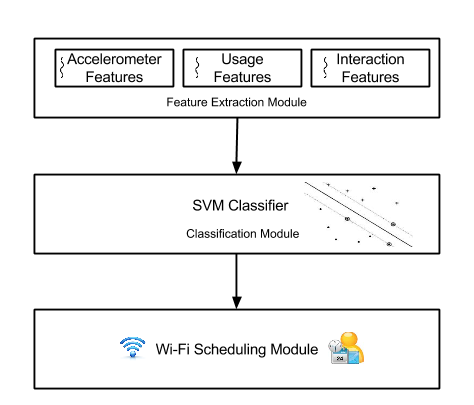
\includegraphics[width=0.9\columnwidth]{ICPR_FLOW_v2.png}
\caption{Primary steps in the algorithm with data flow. Feature extraction module extracts the Accelerometer based, usage based and interaction based features. Classification module predicts the user activity level using SVM Classifier and Wi-Fi Scheduling Module schedules the Wi-Fi state based on the predicted output.}
\label{fig:flow}}
\end{figure}
\end{center}

\section{Classification Frame Work}
%{\bf Move Wi-Fi Sceduling to the previous section}

\subsection{Feature Extraction}
\label{sec:Features}

To extract the data from the smartphone, we created an
Android application that records the required data.
Data was collected over the period of half an hour to
predict the user’s behavior for next cycle. After each
half an hour, the application starts a service to collect the data.
The service runs for the duration of 30 seconds and executes
the following processes.


\begin{enumerate}
\item Partial wake-lock is acquired to prevent smartphone from going to sleep during the process execution.
\item The required data is collected for the duration of 30 seconds.
\item The user activity label is predicted by the classification module from the collected data.
\item The Wi-Fi is scheduled for next half an hour based on the predicted label.
\item Wake-lock is released and phone is allowed to go to sleep.
\end{enumerate}
%The data from the accelerometer and the phone usage patterns are extracted in parallel and used as the features for predicting the user behavior.
We divides the features into three categories- accelerometer based, system usage based and interaction based features. These features are explained in details below.
 
\subsubsection{Accelerometer Based Features}
Accelerometer based features are indication of the physical
activity of the user like stationary, walking, running etc. The assumption behind is if the
user is running or walking the probability of using his phone is much less as compare to
stationary state.

Accelerometer continuously samples the acceleration at the specified sampling interval and produces 3-D acceleration readings $S$ = ($S_X$, $S_Y$, $S_Z$) along X, Y and Z direction. As the acceleration in a direction depends on the orientation of the phone, the overall acceleration $S_\phi$ = $||S_X, S_Y, S_Z||$ is also considered as feature. The sensor reading thus becomes a 4-D vector.
Each device is calibrated differently. So we neglected the acceleration due to gravity while calculating the acceleration of the smartphone.

The accelerometer data is tracked for the user with the sampling frequency of $5Hz$. The accelerometer is tracked for 30 seconds and the following features are extracted. \\
%The segments are formed based on the 1 second interval readings. The frames are formed using 5 consecutive segments. $S$ defines the overall signal observed. $S_I$ denotes the component of $S$ in $I$-th dimension.
%\begin{itemize}
%\item
\emph{Average mean} along $S_X$, $S_Y$, $S_Z$ and the $S_\phi$ vector.
\begin{align*}
\mu_d = \frac{\sum_{i=1}^n S_{d,i}}{n}; d \in \{X, Y, Z, \phi\}
\end{align*}
%\item
\emph{Standard deviation} along $S_X$,$S_Y$,$S_Z$ and the $S_\phi$ vector. Standard deviation indicates the dispersion in the acceleration along different axis.
\begin{align*}
\sigma_d = \sqrt{\frac{\sum_{i=1}^n (S_{d,i} - \mu_d)^2 }{n-1}} ; d \in \{X, Y, Z, \phi\}
\end{align*}
%\item
\emph{Correlation} among each pair of $S_X$, $S_Y$, $S_Z$ and the $S_\phi$ vector. Correlation implies the strength between two corresponding axis signals.
\begin{align*}
r_{d,d'} = \frac{\sum_{i=1}^n (S_{d,i}-\mu_d) \times (S_{d',i}-\mu_{d'}) }{\sqrt{\sum_{i=1}^n (S_{d,i}-\mu_d)^2 \times \sum_{i=1}^n (S_{d',i}-\mu_{d'})^2}} ;
\end{align*}
\begin{align*}
 d,d' \in \{X, Y, Z, \phi\} , d \neq d'
\end{align*}
%\item
\emph{Fourier energy} for $S_X$, $S_Y$, $S_Z$ and the $S_\phi$ vector. The energy feature is the sum of all the squared DFT component magnitudes
except the DC component of the signal as the DC component (mean) has been used as an individual feature. The magnitudes are divided by the number of components for normalization.
\begin{align*}
\varepsilon_d = \frac{1}{n}\sum_{i=1}^n || \mathcal{F}(S_d)_i||; d \in \{X,Y,Z,\phi\}
\end{align*}
%\item
\emph{Fourier entropy} for $S_X$, $S_Y$, $S_Z$ and the $S_\phi$ vector. Fourier entropy is the normalized information present in the DFT of the signal, excluding the DC component.
\begin{align*}
\delta_d = \sum_{i=1}^n ||\mathcal{F}(S_d)_i|| \times log (\frac{1}{|| \mathcal{F}(S_d)_i||})
\end{align*}
%\end{itemize}
The intuition behind using accelerometer based features is that Wi-Fi requirements are different during different activities of the user.

\subsubsection{System Usage Based Features}
System Usage based
features tells how extensively the phone is being utilized.
Features will be higher if
the phone is used for heavy applications like voice calling, network browsing  vs. when the phone is used for viewing SMS, setting alarm etc.

The system usage feature of the smartphone is computed based on the
following entity.

\begin{itemize}
\item The average CPU utilization of the smartphone.
\item The average memory used by the applications in the smartphone.
\end{itemize}
The CPU utilization tells about state of running applications and the memory used tells about the state of installed applications and background services.

\subsubsection{Interaction Based Features}
Interaction based features
tells how frequently user is using his phone. More frequent the
user is on the device, more likely he will requiring the network
connectivity.\\
Interaction based features consist of the following features.
\begin{itemize}
\item \emph{Screen On Time}: In half an hour duration, total time in milliseconds
for which screen was on.
\item \emph{Frequency Of Interactions}: In half an hour duration, total number of interaction (that is number of time the screen has been turned off and turned on) by the user.
\end{itemize}
The features are extracted in parallel so as to get the
consistent data and reduce the battery consumption due to wake-lock acquisition by the application.
Finally we concatenate all the features to form a final feature vector for the classification.

\subsection{Training and Classification}
The user's activity is modeled based on his behavior.
The features extracted by the feature extraction
module is fed to the classification module for prediction.
We classified the user's activity level into four different classes,
labeled by $l_0$, $l_1$, $l_2$ and $l_3$.

\subsubsection{Training}
For training purposes, we created an application
that logs the accelerometer, screen on duration, internet, CPU and RAM usage of the device at every half an hour interval.
We scaled the internet usage based on
the screen on duration in half an hour as well as and the data traffic. The assumption is
if the screen is off and the Wi-Fi is still on then without any data traffic this should
be handled in intelligent way.
We have categorized user into four categories
no usage, low usage, medium usage
and high usage. Class label of a feature vector created during current time window is decided based on the internet usage by the user in next time window.
We run the application for ~7 working days which resulted into 310 feature vector.
For preserving the usability
of the application, the classes are  given different penalty
scores. Table \ref{tab:weights} shows the weights assigned to different classes while training. Weights are calculated in such a way so that(Number of features of a class $\times$ Weight of the corresponding class) should be constant across the classes.


\begin{table}[h]
\begin{center}
\centering{
\caption{Class weights assigned to different activity level while training.}
\label{tab:weights}
\begin{tabular}{| c | c |  c | c | c | c |}
\hline
Class Label &  Very Low ($l_0$) & Low ($l_1$) & Medium ($l_2$) & High ($l_3$) \\
\hline
Weight & 1.0 & 2.71 & 8.92 & 4.92\\
\hline
\end{tabular}}
\end{center}
\end{table}
%The algorithm to turn off the Wi-Fi for the specific duration of time. We used SVM    
\subsubsection{Classification}
For classification, the trained SVM model along with the feature extraction module is deployed on the smartphone. The features are collected for half an hour interval. After half an hour, the prediction (based on the features from feature extraction module) is done. The SVM model created during training is used for predicting the labels. The predicted label is then send to the Wi-Fi scheduling module and the Wi-Fi is scheduled appropriately.

\section{Experimentation and Results}
\label{sec:Exp}

We evaluated our approach based on two metrics, the power saved and the user happiness.
Power saved metric measures the overall power saved by our method. Although the power
saving is important, it should not hamper the user's overall experience on the smartphone.
So user happiness testing is performed to test the user's satisfaction with the software.

For measuring the power saved by our software, we subjected the phones to real-world behaviors (via calls, messages and emails) under two different settings, when our proposed method is installed and when it is not. The percentage drop in the power is computed in both the settings to find the energy efficiency achieved by our method. For finding the user happiness, we installed the application on smartphones of two different users and recorded the number of times they switched the Wi-Fi state manually. Each manual switch is considered as a penalty on user happiness. Section~\ref{sec:Implementation} explains the implementation of the system. Section~\ref{powersaved} shows the power saved by the application and Section~\ref{userhapiness} shows the user happiness scores obtained when the application was installed on user's smartphone.

\subsection{Implementation}
\label{sec:Implementation}
An android application is created for capturing the features, predicting the activity and scheduling the Wi-Fi. The application schedules a prediction service at intervals of half an hour. Along with the service, it also registers a broadcast receiver that listens to screen state change event and logs the changes. After every half an hour, the service wakes the android system and 3D accelerometer readings are recorded for 30 seconds. Based on the readings, the accelerometer signal's mean, standard deviation, correlation and Fourier transform is computed. Along with these features, the screen on time and frequency of interactions are also evaluated using the logs created by the broadcast receiver. Android OS logs the internet, CPU and memory usage of the system. The average internet, CPU and memory usage is calculated based on the logs created by the OS. To maintain consistency among different features, all the features are extracted at the same time. Features are concatenated into a single feature vector. SVM classifier is used to predict the usage in next half an hour (using a pre-trained model) utilizing these features. Based on the predicted output by the classifier (high, medium, low or very low), the Wi-Fi is turned off and an alarm manager is scheduled to turn it on after suitable interval of time. All the decisions made by the classifier are logged for the purpose of evaluation. For evaluating user happiness, all Wi-Fi state changes are also logged. The number of manual state change events are extracted and considered as a measure for calculating user happiness. The activity prediction is shown to be achievable using light-weight computations without consuming much power or memory. Our application took only 5MB of RAM and 101KB external memory, which is similar to the average requirements for an application on smartphones. Also, our application took 1\% of battery in 24 hours\footnote{The power consumed by the application is recorded through battery info manager on android OS.}.

\subsection{Power saved by the software}
\label{powersaved}
User have different activities scheduled at different times. For example, number/durations of calls in one hour might be very different from the number of calls in the next hour. Similarly the power consumed in other tasks like messages, games etc. might be different in the two hours. So, calculating the battery drop in the two corresponding hours (once with the scheduler and once without the scheduler) might not be an accurate measure to evaluate the power saved by our software.

To evaluate the power saving by our software we took two device from both the categories (refer Table \ref{tab:phonespec} for specification) having same set of application, battery state, memory usage etc., and performed below test plan on all four devices, two having our software installed (one from each category) and two without our software. Table~\ref{tab:test} lists the activities carried out on the smartphone. All the activities are performed at almost same time and for same duration. For example, the calls on all the devices are performed simultaneously for 2 minutes duration. Similarly, all the messages and emails are also send simultaneously so that the loss incurred by other processes remains same. The controlled experiment was performed for 4 hours in similar settings and the battery dissipated on each device is recorded. Figure~\ref{fig:bardrop} shows the relative percentage drop in battery on the devices after each hour.

\begin{table}[h]
\begin{center}
{
\caption{Energy Efficiency Testing: Percentage battery dropped in Samsung Galaxy S (Dev.1) and HTC Explorer (Dev.2) during controlled tests.}
\label{tab:test}
%\begin{tabular}{| m{1.1cm} | m{0.95cm} | m{0.8cm} | m{1.1cm} | m{1.0cm} | m{1.0cm} |}
\begin{tabular}{| c | c | c | c | c | c |}
\hline
% &  \bf Messages Received &  \bf Number of Calls  & \bf E-Mails Received-/Replied    & \bf Drop in Battery (Dev.1) & \bf Drop in Battery (Dev.2) \\
 &  \bf Messages &  \bf Number & \bf E-Mails     & \bf Drop in   & \bf Drop in  \\
 &  \bf Received  &  \bf of Calls  & \bf  Received    & \bf Battery & \bf Battery \\
 &   &   & \bf  and Replied    & \bf (Dev.1) & \bf (Dev.2) \\
\hline
\bf Without & \multirow{2}{*}{25} & \multirow{2}{*}{15} & \multirow{2}{*}{25} & \multirow{2}{*}{38\%} & \multirow{2}{*}{52\%} \\
\bf Scheduler &  &  &  &  &  \\
\hline
\bf With & \multirow{2}{*}{25} & \multirow{2}{*}{15} & \multirow{2}{*}{25} & \multirow{2}{*}{28\%} & \multirow{2}{*}{15\%} \\
\bf Scheduler & & & & &  \\
\hline
\end{tabular}}
\end{center}
\end{table}

%%%%%%%%%%%%%%%%%%%%%%%%%%%%%%%%%%%%%%%%%%%%%%%%%%%%%%%%%%%%%%%%%%%%%%%%%%%%%%%%%%%
\begin{table}[h]
\centering
\caption{User Happiness: Count of Number of times Wi-Fi was manually turned on.}
\label{tab:user_happiness}
\begin{tabular}{|>{\centering}m{1.5cm}| >{\centering}m{1.1cm}|>{\centering}m{1.25cm} |>{\centering}m{1.1cm}|>{\centering}m{1.25cm}|>{\centering}m{1.1cm}|>{\centering}m{1.25cm}|>{\centering}m{1.1cm}|>{\centering}m{1.25cm}|}
\hline
 & \multicolumn{2}{|m{2.2cm}|} {Wi-Fi turn-on count (Usr 1)} &  \multicolumn{2}{|m{2.2cm}|} {\% Battery Drop (Usr 1)} &\multicolumn{2}{|m{2.2cm}|} { Wi-Fi turn-on count (Usr 2) } & \multicolumn{2}{|m{2.2cm}|} { \% Battery Drop (Usr 2)} \tabularnewline
\hline
& Working Hrs. & Non-Working Hrs. & Working Hrs. & Non-Working Hrs. & Working Hrs. & Non-Working Hrs. & Working Hrs. & Non-Working Hrs.
\tabularnewline
\hline
{\bf Without Scheduler} & \centering NA & NA &\centering 38 & 26 & \centering NA & NA & {\centering 33} & 8 \tabularnewline
\hline
{\bf With Scheduler} & \centering 5 & 2 & \centering 29 & 19 & \centering 3 & 0 & {\centering 13} & 7\tabularnewline
\hline
\end{tabular}
\end{table}
%%%%%%%%%%%%%%%%%%%%%%%%%%%%%%%%%%%%%%%%%%%%%%%%%%%%%%%%%%%%%%%%%%%%%%%%%%%%%%%%%%%%%


\begin{center}
\begin{figure}[!ht]
\centering{
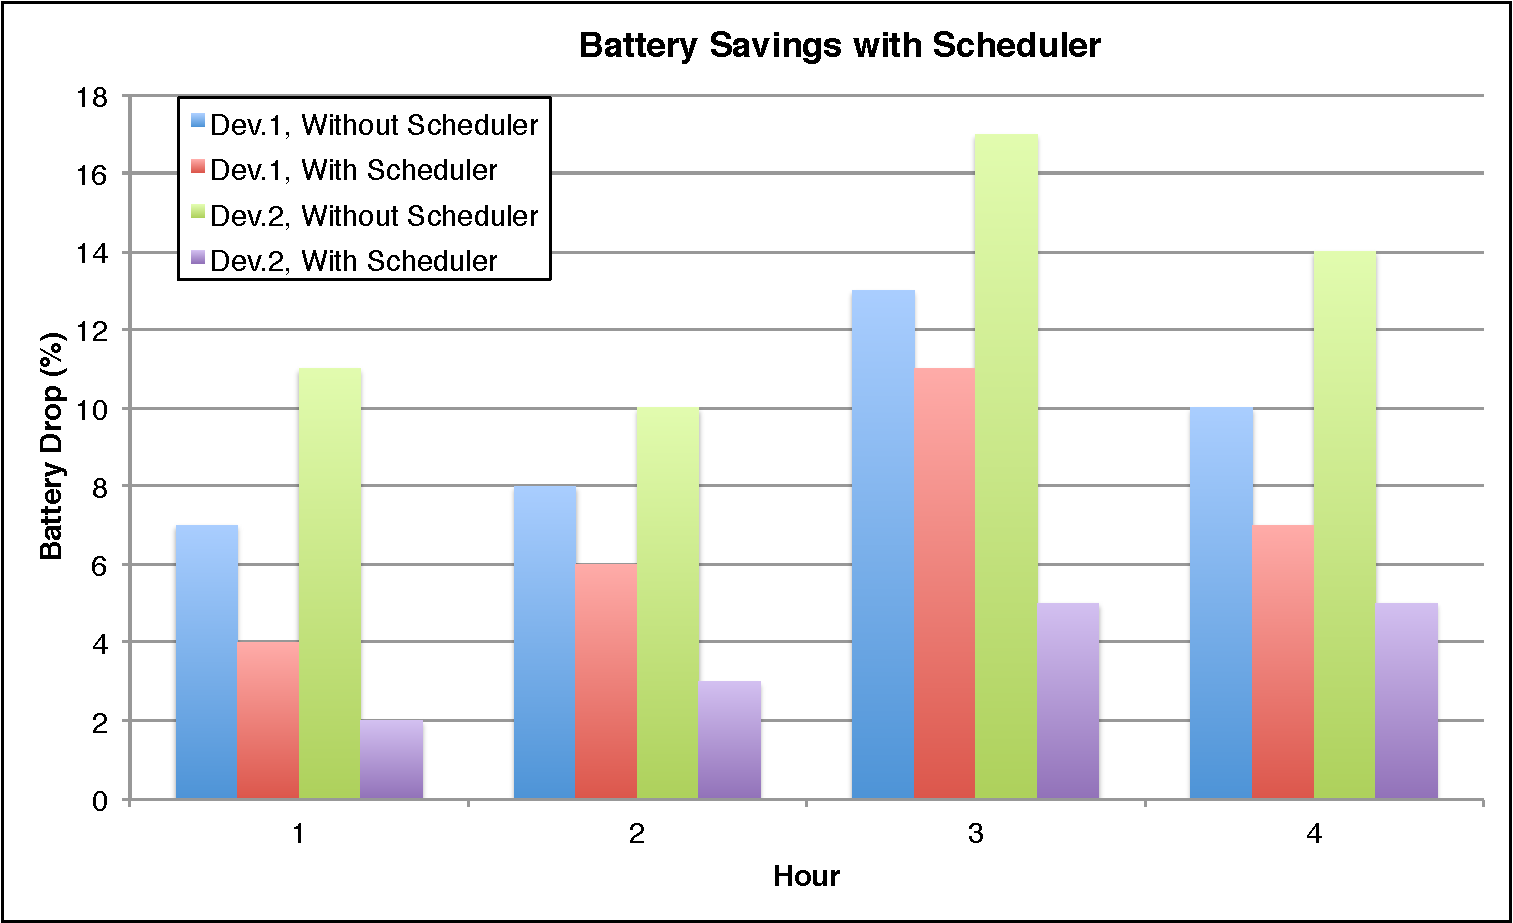
\includegraphics[width=1\columnwidth]{BatterySavings.pdf}
\caption{Percentage drop in battery with time under different settings (Dev.1 and Dev.2).}
\label{fig:bardrop}}
\end{figure}
\end{center}

%%%%%%%%%%%%%%%%%%%%%%%%%%%%%%%%%%%%%%%%%%%%%%%%%%%%%%%%%%%%%%%%%%%%%%%%%%%
\begin{table}[h]
\caption{Specifications of the phones on which testing was conducted.}
\label{tab:phonespec}
\makebox[\textwidth]{
\begin{tabular}{|m{1.3cm}| m{1.9cm}| m{3.4cm}| m{3.4cm}| m{3.4cm}|}
\hline
& \bf Feature & \bf Dev.1: Samsung & \bf Dev.2: HTC & \bf Dev.3: Asus\\
\hline
 \bf General & 2G, 3G Freq &  GSM, HSDPA, Mini & GSM, HSDPA, Mini & as1 \\
\hline
\bf Display & Type, Size & AMOLED capacitive touch, 4.0" & TFT capacitive touch, 3.2" & as1 \\
\hline
\bf Memory & Internal & 512 MB RAM, 512 MB ROM & 512 MB RAM, 512 MB ROM & as1 \\
\hline
\bf Data & [GPRS], [EDGE], [Speed], [WLAN], [Bluetooth], [USB] & [ Class 12 (4+1/3+2/2+3/1+4 slots), 32 - 48 kbps], [Class 12], [ HSDPA, 14.4 Mbps; HSUPA, 5.76 Mbps], [Wi-Fi 802.11 b/g/n, DLNA, Wi-Fi hotspot ], [Yes, v3.0 with A2DP], [Yes, microUSB v2.0] & [ Up to 80 kbps], [Up to 236.8 kbps], [ HSDPA, 14.4 Mbps; HSUPA, 5.76 Mbps], [Wi-Fi 802.11 b/g/n, DLNA, Wi-Fi hotspot ], [Yes, v3.0 with A2DP,EDR], [Yes, microUSB v2.0]
 & as1 \\
\hline
\bf Features & [OS], [Chipset], [CPU], [GPU], [Sensors], [Messaging] & [Android OS, v2.3 (Gingerbread)], [Qualcomm MSM8255T Snapdragon], [1.4 GHz Scorpion], [Adreno 205], [Accelerometer, proximity, compass],[SMS(threaded view), MMS, Email, Push Mail, IM, RSS] & [Android OS, v2.3 (Gingerbread)], [Qualcomm MSM8255T Snapdragon], [ 600 MHz Cortex A5], [Adreno 200], [Accelerometer, proximity],[SMS(threaded view), MMS, Email, Push Mail, IM, RSS] & as1 \\
\hline
\end{tabular}
}
\end{table}
%%%%%%%%%%%%%%%%%%%%%%%%%%%%%%%%%%%%%%%%%%%%%%%%%%%%%%%%%%%%%%%%%%%%%%%%%%%%%%%%%%


\subsection{Measuring User Happiness}
\label{userhapiness}
Power saving is important but at the same time
we have to take care that user experience should not be hampered a lot. To verify this
we conducted an experiment in which we have given our software to users and logged there
battery usage in two categories first when the user is very active second when the user
is less active. Along with battery usage, the number of times the Wi-Fi state is changed manually is also recorded. Each Wi-Fi switch by the user is considered as misclassification by the algorithm. The higher the number of switches by the user, the more unhappy the user is with the application.
Table \ref{tab:user_happiness} shows 6 hrs analysis when the user is highly active (working hours) and shows the 6 hrs analysis when the user is not much active (non-working hours) on the smartphone device.
Our application took just 1\% of battery in 24 hours and saved 10 to 37\% of battery in 4 hours without much affecting
user convenience. The battery usage vs. amount of battery saved confirms that the application can be used non-stop and can save significant amount of power, especially for heavy internet users.



\section{Experiment Extended}
We further extend the experiments and benchmark the performance of different machine learning algorithms with fresh dataset using same software as Section \ref{sec:Exp} by porting it on a ASUS low cost smart phone Table \ref{tab:phonespec}. We did the comparitive study of the three algorithms \textit{kNN, SVM and Neural Networks} on the newly collected dataset. 
%%by benchmarking the by replicating the same set of experiments like power saved and user happiness as perfomed in previous Section \ref{sec:Exp}.

\subsection{Dataset Collection and Hyperparameter Tuning}
We followed exactly the same process for the dataset generation as done in previous Section \ref{sec:Exp}. After
every \textit{30 mins}, the software service wakes up the android system and log all the necessary information like 3D accelerometer readings, screen on time, frequency of interaction, CPU and memory usage of the system are also logged using broadcast receiver and Android OS logs. By following these steps we run the application for ~20 working days which resulted into 956 feature vectors. Parameter tuning is carried by spliting the dataset in train and validation in 80-20 ratio.
\subsubsection{\textit{k}NN Paramaeter Tuning}
In a \textit{k}NN algorithm number of neighbors(\textit{k}) is a hyper parameter that need to be tune for model building. No optimal number of neighbors suits all kind of data sets, individual dataset has it's own requirements. The small value of \textit{k} leads to noise will have a higher influence on the result where as large value of \textit{k} make it computationally expensive. Figure \ref{fig:knn_err} mean error rate for different values of \textit{k} ranging from 1 to 30. For our model selection we have chosen \textbf{\textit{k = 7}} as it seems to be good balance between the noise and the cost of computation.

\begin{center}
\begin{figure}[!ht]
\centering{
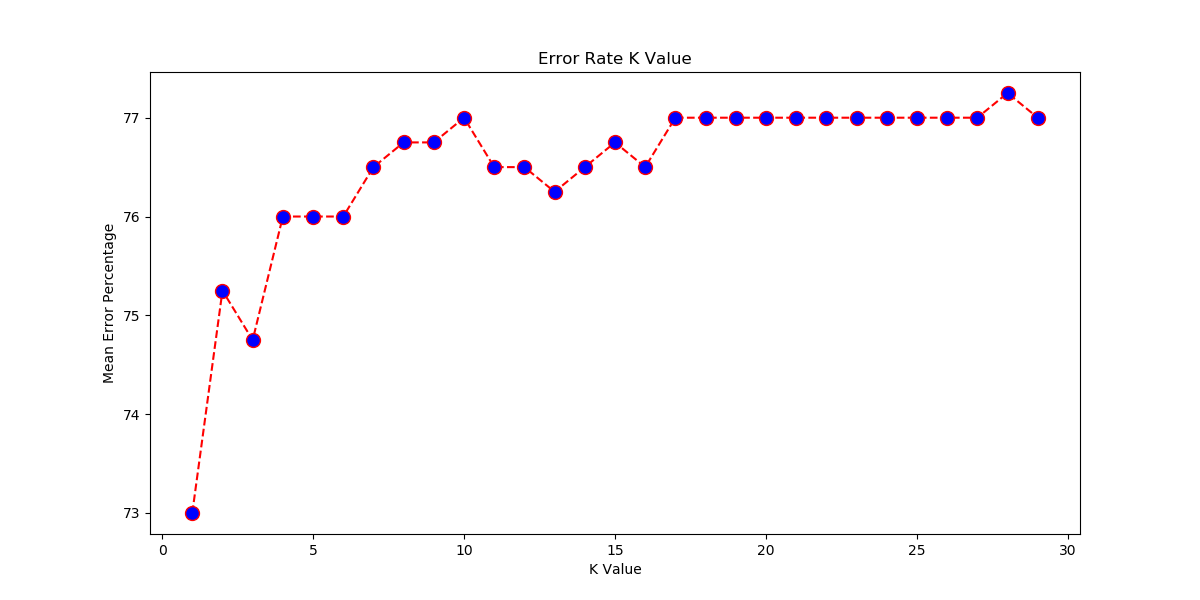
\includegraphics[width=0.9\columnwidth]{knn_err.png}
\caption{Tuning number of neigbours(\textit{k}). We vary \textit{k} from 1 to 30 and report the mean error on the validation set. We can see after \textit{k} = 16 the error rate is almost constant which indiactes absence of noise in the model.}
\label{fig:knn_err}}
\end{figure}
\end{center}

\subsubsection{SVM Parameter Tuning}
C and Gamma are the parameters for a nonlinear support vector machine(SVM) with a Gaussian radial basis function kernel. We ran grid search algorithm to find optimal C and Gamma pair for our SVM model(Figure \ref{fig:svm_param_tuning}). We build our model \textit{C=8} and \textit{Gamma=0.3125} and achieved 84.7\% accuracy with 10-fold cross validation process. 

\begin{center}
\begin{figure}[!ht]
\centering{
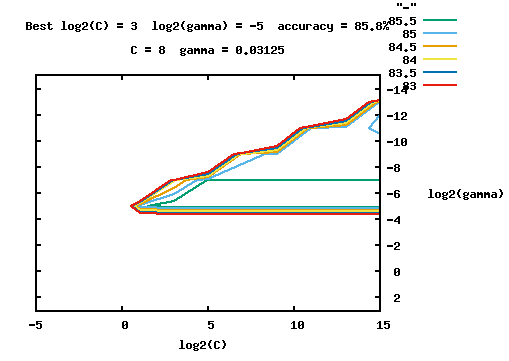
\includegraphics[width=0.8\columnwidth]{svm_param_tuning.png}
\caption{Grid search on the dataset to find the optimal C and Gamma pair for the SVM model.}
\label{fig:svm_param_tuning}}
\end{figure}
\end{center}


\subsubsection{Neural Networks Paramaeter Tuning} While training a neural network we have to make many decisions regarding the following hyperparameter those are (i) \textit{Solver} (ii) \textit{Number of hidden layers} and \textit{Number of hidden units for each hidden layer} (iii) \textit{Learning rate }. We have used scit-learn framework~\cite{scite_learn_framework} to tune these hyperparameters.

\textbf{Solver:} The default solver \textit{adam} for the scikit-learn works good with relatively large dataset with thousands of training samples. For small dataset \textit{lbfgs} converge faster and perform better~\cite{scite_learn_framework}. In all our experiments we have used \textit{lbfgs} solver.

\textbf{Number of Hidden Layers and Hidden Units:} We have two decesions to made (i) \textit{How many hidden layers} (ii) \textit{How many units in each hideen layer}. We will first fix the number of hidden layer to use in neural network. From \textit{Introduction to Neural Networks for Java, second edition} by \textit{Jeff Heaton} summarizes the capabilities of neural network architectures(\cite{hilton_web_archive}) with various hidden layers like Table \ref{tab:no_hdn_layer}. In our experiments we have considered one hidden layer for our model. A neural network model with one hidden layer is capable enough for continous maping between two spaces(Table\ref{tab:no_hdn_layer}). Deciding number of hidden layers is only a small part we shold also fix the the number of neurons in each hidden layer. Using too few neurons in the hidden layers will lead underfitt where as too many neurons can overfitt the model. In order to find the right number of neurons in hidden layer cross-validation accuracy mechanism were used.

\begin{table}[h]
\centering


\begin{tabular}{|P{1.3cm}| P{12.0cm}|}

\hline
\bf No Hidden Layer & \bf Result \\
\hline
0 & Only capable of representing linear separable functions or decisions. \\
\hline
1 & Can approximate any function that contains a continuous mapping from one finite space to another. \\
\hline
2 & Can represent an arbitrary decision boundary to arbitrary accuracy with rational activation functions and can approximate any smooth mapping to any accuracy. \\
\hline
$>$2 & Additional layers can learn complex representations (sort of automatic feature engineering) for layer layers. \\
\hline
\end{tabular}

\caption{Hidden layer units capability to capture data distribution.}
\label{tab:no_hdn_layer}
\end{table}

\textbf{Learning rate:} Learning rate is one of the most significant hyperparameter for neural netowrks. We cannot analytically calculate the optimal learning rate for a given model and dataset. Instead optimal learning rate must be discovered via trial and error. We have tried several combination of learning rate with other hyperparameters.

To train our model we have tried varying number of hidden units ranging from 6 to 28 along with different learning rates 0.1, 0.01 and 0.005. Figure \ref{fig:learning_rate_hiddenlayer01} shows the results for the train and validation set accuracy. From the figure~\ref{fig:learning_rate_hiddenlayer01} we can observe both validation and train dataset accuracy increases with the number of hidden units upto certian number. Further increase in hidden units has no effect on validation accuracy where as train accuracy keeps on increasing and overfit the model. Neural netowrk model with \textit{ hidden units = 18, learnin rate = 0.005} achieved \textit{train accuracy = 74.1 and validation accuracy = 72.3} which seems to be best balance between the model complexity and accuracy.
%%%%%% Original Features VS Useful Features %%%%%%%%%%%%%%
\begin{figure}[h]
\centering
\subfloat[ ]{ 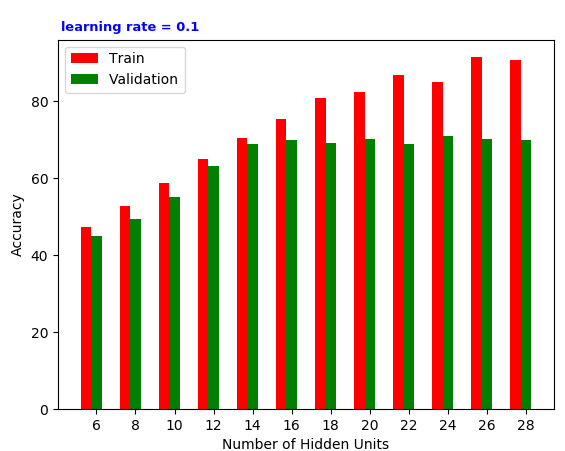
\includegraphics[width=5.7cm,height=4.5cm]{lr01_hidden_layer01}}
\subfloat[ ]{ 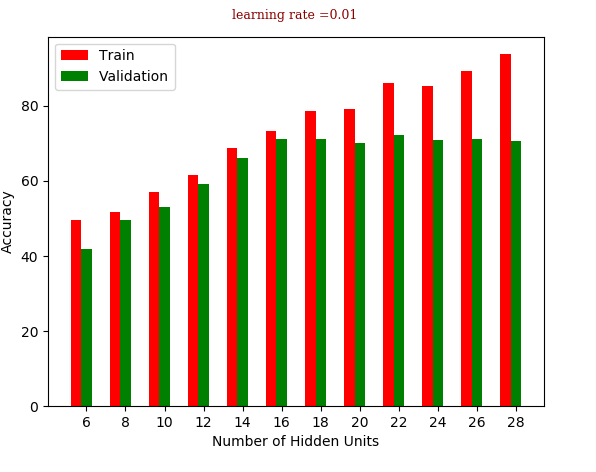
\includegraphics[width=5.7cm,height=4.5cm]{lr02_hidden_layer01}}
\subfloat[ ]{ 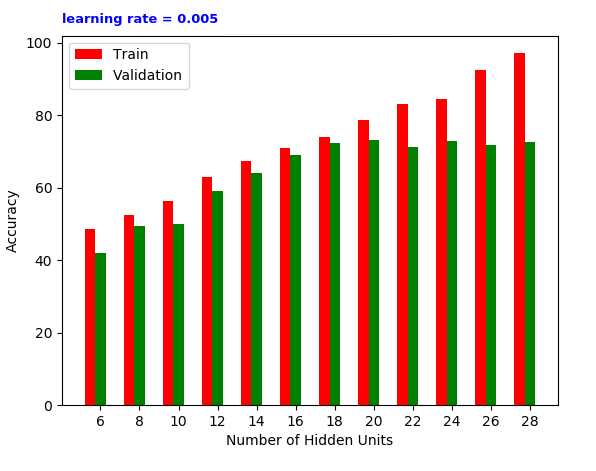
\includegraphics[width=5.7cm,height=4.5cm]{lr03_hidden_layer01}}
\caption{Original image features (a) vs those features which could 
be considered useful features (b). Transient objects, occlusions in the 
foreground and non-distinctive areas of the scenes are found to 
be without useful features.}
\label{fig:learning_rate_hiddenlayer01}
\end{figure}
%%%%%%%%%%%%%%%%%%%%%%%%%%%%%%%%%% 
\subsubsection{Results}


\section{Summary}
Power consumption and the consequent low battery life is one of the primary limiting factors for modern mobile devices.
In this work, we proposed an effective way to nullify some of this problem by predicting user activity levels and scheduling
the power hungry wireless modules accordingly. The encouraging results of the experiments lead us to affirm that a step
forward has been taken to personalize the equipment so that it can function well while improving power efficiency.

The effectiveness of the proposed approach can be improved and extended in many ways. Application time interval
can be scheduled dynamically, making it adaptive to user's activity level, which should give better result in terms of user happiness
as well as battery saving. As the application is monitoring and modeling the user's activity, it can also perform additional tasks
such as silencing the phone between meeting/sleep hours, or put the phone in silent mode when the user is driving.
